\documentclass{article}
\usepackage[utf8]{inputenc}
\usepackage{amsmath}
\usepackage{kotex}
\usepackage{graphicx}

\begin{document}

\section{Exercise 1}
\begin{center}
    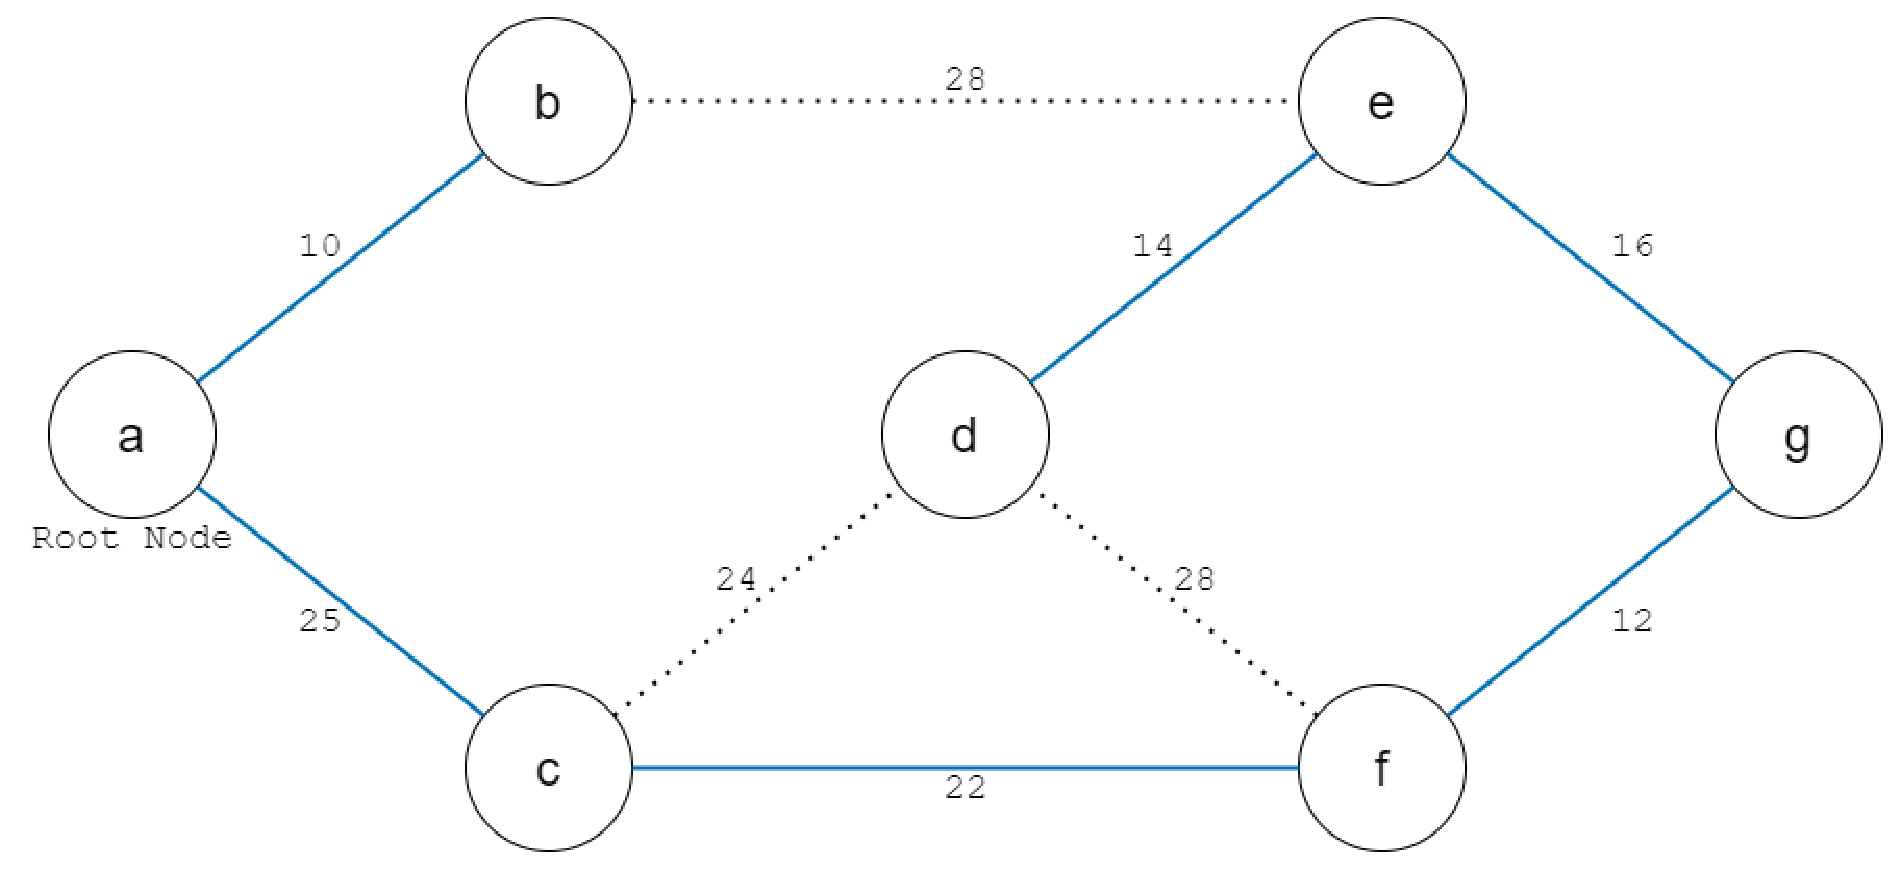
\includegraphics[scale=.4]{./img/prim_algo.eps}
\end{center}
프림 알고리즘을 실행할 때에 있어서, a를 root node로 지정하였다.
파란색 간선의 집합이 MST 이며, 총 weight는 99 이다.

\section{Exercise 3}
\subsection{}
Weight가 같은 간선이 있다면, MST가 유일하지 않을 수 있다. 왜냐하면 weight가 같은 간선 중, 어느 하나를 선택하더라도
그래프의 총 weight는 같기 때문이다. 따라서 강의 노트에서와 같이 'e-c', 'e-f' 간선 둘 다 총 weight는 같으면서, 동시에 MST 조건을 만족하는 경우가 발생할 수 있다.
\subsection{}
귀류법을 통해서 증명해 보고자 한다.

주어진 그래프 $G=(V, E)$의 서로 다른 MST인 $T_1 = (V, E_1)$과 $T_2 = (V, E_2)$가 있다고 가정해보자.
이 때, vertex $A$와 $B$를 지나는 간선 $e$가 그래프 $G$에서 가장 낮은 weight를 가졌다고 가정한다.
또한 간선 $e$는 $T_1$에 포함되어 있지만, $T_2$에는 포함되어 있지 않다고 가정한다.
그러면 $T_2$는 $T_1$에는 포함되지 않는 간선 $e'$를 최소한 한개 이상 가지게 될 것이다.

만약 $e$를 $T_2$에 포함시킨다면, cycle이 생겨날 것이다.
이 때, $T_2$에서 $e$를 $e'$과 서로 바꾼다면 $e_1 \cup T_2 - e_2$를 얻게 되는데, 이는 spanning tree의 조건은 만족하지만 $T_2$ 보다 낮은 weight를 갖게 된다.
이는 모순으로, $T_2$는 존재할 수 없다. 따라서 $G$의 MST는 $T_1$ 뿐 만이 유일하다고 할 수 있다.

\end{document}
